\mysection{АНАЛИЗ ПРЕДМЕТНОЙ ОБЛАСТИ}
\subsection{Встроенные системы}
\label{subsec:linux-for-embedded-systems}

\textbf{Встроенные вычислительные системы} (ВВС) – специализированные (заказные) вычислительные системы (ВС), непосредственно взаимодействующие с объектом контроля или управления и объединенные с ним единой конструкцией \cite{EMBEDDED}.

В силу специфики использования, обычно встроенные системы имеют низкое энергопотребление, предназначены для выполнения определенного набора задач и не являются универсальной вычислительной платформой, такой как компьютеры. По этим причинам, многие встроенные системы не используют операционную систему. Тогда программист проводит собственную разработку всего программного обеспечения, которое управляет оборудованием, практически не задействовав многозадачность и взаимодействие с пользователем. Программное обеспечение в таком случае работает непосредственно с оборудованием встроенной системы.

Однако в современном мире существуют более сложные встроенные системы, с расширенным списком решаемых задач.
В такой многозадачной системе, должны быть реализованы следующие механизмы:
\begin{itemize}
  \item распределение памяти;
  \item предоставление времени ЦП разным потокам, процессам;
\end{itemize}

В таком случае программист может использвать ОС, это подход позволяет сосредоточиться на решении задачи, возложенной на ВВС, делегировав управление аппаратными средствами ОС.

Однако операционные системы очень трудно создавать, и это приводит к увеличению количества строк кода в проекте.
При этом важно отметить, что влияние на количество ошибок в коде оказывает количество строк, то есть чем больше строк, тем больше ошибок \cite{EMBEDDED}.
По этой же причине уст­ра­не­ние всех оши­бок в прак­ти­че­ски зна­чи­мом ПО слиш­ком тру­до­ём­ко, вме­сто это­го при его соз­да­нии обыч­но пы­та­ют­ся дос­тичь мак­си­маль­но воз­мож­но­го при за­дан­ных за­тра­тах уров­ня ка­че­ст­ва, как мож­но боль­ше сни­зить ве­ро­ят­ность про­яв­ле­ния оши­бок и ущер­ба от них.
Так как операционные системы развиваются и поддерживаются в течение долгого периода времени\cite{TANENBAUM}, то во встроенных решениях часто используют уже существующие ОС.

\newpage
\subsection{Linux во встроенных системах}

Большое распространение во встроенных системах получили ОС на основе Linux.

\textbf{Дистрибутив Linux} - это операционная система, в основе которой лежит ядро Linux и, зачастую, система управления пакетами.
Дистрибутив может быть представлен в виде предварительно скомпилированных двоичных файлов и пакетов, собранных сопровождающими дистрибутива, или в виде источников в сочетании с инструкциями о том, как их скомпилировать.

Среда разработки в программировании встроенных систем обычно сильно отличается от сред тестирования и производства, они могут использовать разные архитектуры чипов, программные стеки и даже операционные системы.
Во встроенных системах, поскольку аппаратная платформа зачастую выполняется на заказ, разработчик ОС обычно предпочитает генерировать дистрибутив с нуля, из источников.

Как правило, дистрибутив состоит из полного образа программного обеспечения для целевого устройства, включая ядро, драйверы устройств, библиотеки, прикладное программное обеспечение и загрузчик.


\newpage
\subsection{Обзор существующих систем сборки}
В настоящее время существует достаточно большое количество систем, реализующих сборку Linux дистрибутивов для встроенных систем.

\textbf{Система сборки embedded linux} - механизм для построения создания Linux дистрибутивов, обладающий следующими свойствами:
\begin{itemize}
  \item позволяет указать архитектуру оборудования;
  \item позволяет интегрировать приложения пользовательского пространства в образ;
  \item разрешает параллельную сборку;
  \item включает набор инструментов для кросс компиляции;
\end{itemize}

Системы сборки нацелены на решение задачи создания образа Linux дистрибутива.
В рамках проведённого обзора были рассмотрены популярные продукты, позволяющие осуществлять сборку дистрибутивов Linux:
\begin{itemize}
  \item \textbf{Open Embedded/Yocto} -- система для создания полных встроенных изображений с нуля. Используется проектом Yocto в качестве системы сборки.
  \item \textbf{Buildroot} -- система сборки, направленная на простоту использования.
  \item \textbf{Системы адаптации дистрибутивов} -- системы, удалющие ненужные компоненты из настольных дистрибутивов.
\end{itemize}
\newpage
\subsubsection{Open Embedded/Yocto}
Проект Yocto определяется как «проект с открытым исходным кодом, который предоставляет шаблоны, инструменты и методы, помогающие создавать пользовательские системы на основе Linux для встроенных продуктов независимо от аппаратной архитектуры»\cite{YOCTO}.
Это набор рецептов, конфигурационных файлов и зависимостей, используемых для создания пользовательского образа Linux, адаптированного к конкретным пользовательским потребностям.
Yocto использует Openembedded в качестве своей системы сборки.
Технически это два отдельных проекта, названия проектов часто используются взаимозаменяемо.
Результат сборки в целом состоит из трех компонентов:
\begin{itemize}
  \item \textbf{Целевые двоичные файлы} -- к ним относятся загрузчик, ядро, модули ядра, образ корневой файловой системы и любые другие вспомогательные файлы, необходимые для развертывания Linux на целевой платформе.
  \item \textbf{Хранилище пакетов} -- это набор пакетов программного обеспечения, доступных для установки на устройство.
Есть возможность выбрать формат пакета (например, deb, rpm, ipk) в зависимости от потребностей.
Некоторые из них могут быть предварительно установлены в целевые исполняемые файлы, однако можно создавать пакеты для установки в развернутую и функционирующую систему.
Все части rootfs являются пакетами (рис.~\ref{fig: yocto}).
  \item \textbf{Целевая SDK} --  это набор библиотек и заголовочных файлов, представляющих программное обеспечение, установленное на вашей целевом устройстве.
Заголовочные файлы используются разработчиками приложений при создании своего кода, чтобы гарантировать, что они связаны с соответствующими библиотеками.
\end{itemize}

\begin{figure}[h!]
  \centering
  \setlength{\fboxsep}{5pt}
  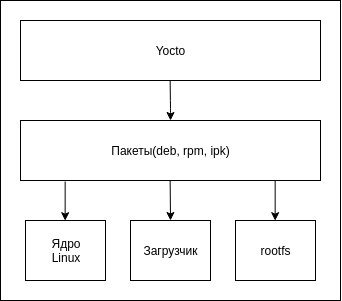
\includegraphics[height=8cm]{build/images/yocto}
  \caption{Структура yocto образа}\label{fig: yocto}
\end{figure}

Проект Yocto широко используется в отрасли и имеет поддержку многих влиятельных компаний. Кроме того, у этого есть большое и энергичное сообщество разработчиков и экосистема, способствующая этому. Сочетание энтузиастов с открытым исходным кодом и корпоративных спонсоров помогает вести проект\cite{YOCTO}.

\textbf{Преимущества использования Yocto:}
\begin{itemize}
  \item Проект легко расширяется через \textbf{слои}, которые можно публиковать независимо для добавления дополнительных функций или для хранения настроек, уникальных для целевой системы.
  \item Широкая поддержка со стороны многих производителей полупроводников и плат.
  \item Настройки для отдельного приложения могут храниться в слое для инкапсуляции и изоляции. Настройки, уникальные для слоя, как правило, хранятся как часть самого слоя, что позволяет применять одни и те же настройки одновременно к нескольким системным конфигурациям.
  \item Yocto также предоставляет четко определенный уровень приоритета задач и возможность их переопределения. Это позволяет определить порядок применения слоев и поиска метаданных. Это также позволяет переопределить настройки в слоях с более высоким приоритетом.

\textbf{Недостатки использования Yocto:}
\end{itemize}
\begin{itemize}
  \item Время сборки и ресурсы разработки достаточно высоки\cite{YOCTO}. Так как количество пакетов, которые необходимо собрать, является значительным, а сборка происходит в несколько потоков. Рабочие станции для разработчиков Yocto, как правило, представляют собой большие системы. Однако, в Yocto имеется встроенный механизм кэширования, который позволяет повторно использовать ранее созданные компоненты, когда параметры для создания определенного пакета не изменились.
\end{itemize}
\newpage
\subsubsection{Buildroot}
Проект Buildroot это «простой, эффективный и простой в использовании инструмент для генерации встроенных систем Linux посредством кросс-компиляции»\cite{BUILDROOT}.
Он разделяет многие из тех же целей, что и проект Yocto, однако он сфокусирован на простоте использования.
По умолчанию Buildroot отключит все необязательные настройки времени компиляции для всех пакетов, что приведет к созданию образа с минимальным объемом.
Разработчик системы должен будет включить настройки, необходимые для его встроенной системы.

Buildroot собирает все компоненты из исходного кода, но не поддерживает управление пакетами. Нет механизма для установки новых пакетов в работающую систему.
Результат сборки в целом состоит из трех компонентов:
\begin{itemize}
  \item \textbf{Основные модули} -- ядро, загрузчик и модули ядра, соответствующие целевому оборудованию(рис.~\ref{fig:buildroot}).;
  \item \textbf{rootfs} -- образ корневой файловой системы и любые другие вспомогательные файлы, необходимые для развертывания Linux на целевой платформе;
  \item \textbf{Набор инструментов,} которые использовалась для сборки всех целевых двоичных файлов;
\end{itemize}

\begin{figure}[h!]
  \centering
  \setlength{\fboxsep}{5pt}
  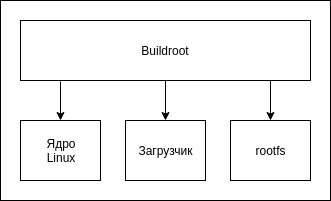
\includegraphics[height=8cm]{build/images/buildroot}
  \caption{Структура buildroot образа}\label{fig:buildroot}
\end{figure}

\textbf{Преимущества использования Buildroot:}
\begin{itemize}
  \item Базовая система сборки написана на Make\cite{BUILDROOT} и достаточно коротка, чтобы позволить разработчику понять всю систему, в то же время будучи достаточно расширяемой для удовлетворения потребностей разработчиков встраиваемых Linux-систем;
Ядро Buildroot обычно обрабатывает только общие случаи использования, но его можно расширять с помощью сценариев;
  \item Система Buildroot использует для своей конфигурации Makefile и язык Kconfig\cite{BUILDROOT}. Kconfig был разработан сообществом разработчиков ядра Linux\cite{KCONFIG} и широко используется в проектах с открытым исходным кодом, что делает его знакомым для многих разработчиков;
  \item В связи со способом сборки, заключающейся в отключении всех необязательных настроек для каждого отдельного пакета, Buildroot обычно создает наименьшие по объему возможные образы с использованием готовой конфигурации.
Время сборки и сборки ресурсов хоста в целом также будет меньше, чем с использованием Yocto;
\end{itemize}

\textbf{Недостатки использования Buildroot:}
\begin{itemize}
  \item Акцент на простоте и минимальных включенных параметрах сборки подразумевает, что разработчику может потребоваться выполнить объемную настройку сборки для пакета, если используется нестандартная конфигурация. Кроме того, все параметры конфигурации для пакета хранятся в одном файле\cite{BUILDROOT}, а это означает, что если проект поддерживает несколько аппаратных платформ, разработчику нужно будет вносить изменения в каждую настройку для каждой платформы;
  \item Любое изменение в файле конфигурации системы требует полной пересборки всех пакетов;
\end{itemize}

\newpage
\subsubsection{Системы адаптации дистрибутивов}
Распространенный подход к проектированию встраиваемых систем на основе Linux заключается в том, чтобы начать с настольного дистрибутива, такого как Debian или Red Hat, и удалять ненужные компоненты, пока установленный образ не поместится в пространство целевого устройства\cite{ARMBIAN}. Это подход, принятый для популярного дистрибутива Raspbian для платформы Raspberry Pi.

\textbf{Преимущества использования cистемы адаптации дистрибутивов:}
\begin{itemize}
  \item Основным преимуществом этого подхода является ознакомленность разработчика с содержимым дистрибутива.
Часто разработчики встраиваемых Linux-систем также являются пользователями настольных Linux-систем и хорошо разбираются в своем дистрибутиве.
Использование аналогичной среды на цели может позволить разработчикам начать работу быстрее.
В зависимости от выбранного дистрибутива, многие дополнительные инструменты могут быть установлены с использованием стандартных пакетных менеджеров, таких как apt и yum;
  \item Количество пакетов в репозиториях пакетных менеджеров, большинства настольных дистрибутивов, обычно больше, чем рецептов для Yocto или Buildroot;
  \item Благодаря встроенному менеджеру пакетов, такой дистрибутив удобно использовать во время разработки продукта в качестве отладочного окружения;
\end{itemize}

\textbf{Недостатки использования cистемы адаптации дистрибутивов:}
\begin{itemize}
  \item Получить воспроизводимую среду таким способом сложно так как поставщики пакетов могут обновлять их версии;
  \item Добавление и удаление пакетов вручную подвержено ошибкам;
\end{itemize}

\newpage
\subsection{Постановка задач исследования}
В рамках данной работы требуется спроектировать и реализовать программное обеспечение для сборки дистрибутивов операционных систем на основе Linux для встроенных систем.

Для достижения поставленной цели необходимо решить следующие задачи:
\begin{itemize}
  \item определить требования к системе;
  \item спроектировать архитектуру системы;
  \item реализовать программное обеспечение системы в соответствии с разработанной архитектурой;
  \item провести тестирование и апробацию;
\end{itemize}
\newpage
